%\setcounter{chapter}{44}
\chapter{How to Give Talks\index{Talks}}
\label{chapter:how_to_give_talks}

\section{Introduction}
Giving good talks is important for people who use the material of this book--for students, researchers, and engineers.
One  might think,  ``It is the work itself that really counts.  Giving a talk about it is secondary.''
But the ability to give a good talk is like having a big serve in tennis—by itself, it doesn’t win the game for you, but it sure helps.  And the very best tennis players all have great serves.  So we include in this chapter material that we have found helpful in giving talks.

There are many other sources for giving talks, and you should access several of them to pick out the tips that work best for you.  Prof. Patrick Winston's talk about giving talks is great \cite{WinstonSpeaks}, and another good source is this book \cite{Hoogterp}.   This chapter has heuristics that have worked well for us.

\subsection{A Taxonomy of Talks}

There are different kinds of talks.  Conference and workshop talks may range in length between 3 minutes for a ``fast-forward'' talk to 45 or 60 minutes for a keynote address.  You may be one of many speakers, sometimes speaking in different rooms at the same time.
Sometimes you will visit a university or company and speak in a special seminar. (Here \cite{MITFacultyJobTalks2022} is a list of tips regarding faculty job talks from the MIT faculty.)

It is very often the case that the audience will have a wide range of familiarity with the work and topic that you will present about.  In a small seminar to a competing research group, there may be many people who are very familiar with your work.  But even in such a small seminar, and especially to a larger group, there may be many people who don't know your area, nor perhaps not even your broad area.  So you will to include material to let the uninitiated not be lost.  Even people who are very  familiar with the topic will appreciate hearing material they already understand presented clearly and well.  

The tips in the chapter apply to talks of all lengths.  However, one class of talks is so short as to be a special case:  the very short talk.

\section{Very Short Talks (2 -- 10 minutes)}
Short talks are often advertisements, designed to persuade the listener to read your paper, or to listen to a longer version of the talk.  Rather than trying to convey many details about your work, you should aim to have the audience remember the main idea behind your work, and to share your excitement about the work.

For five minute talks describing students' final project class presentations, we suggest that the students cover these points:
\begin{enumerate}
\item What problem did you address?
\item Why is it interesting?
\item Why is it hard?
\item What was the key to your approach?
\item How well did it work?
\end{enumerate}
That structure can be used for other short talks, too.
For very short talks, the time needed to go through the whole thing is minimal, and there is no excuse not to practise the talk, from start to finish, several times.  Next, we cover points that we feel relate to all types of technical talks, regardless of length.


\section{Preparation}

\begin{figure}[htpb!]
\centerline{
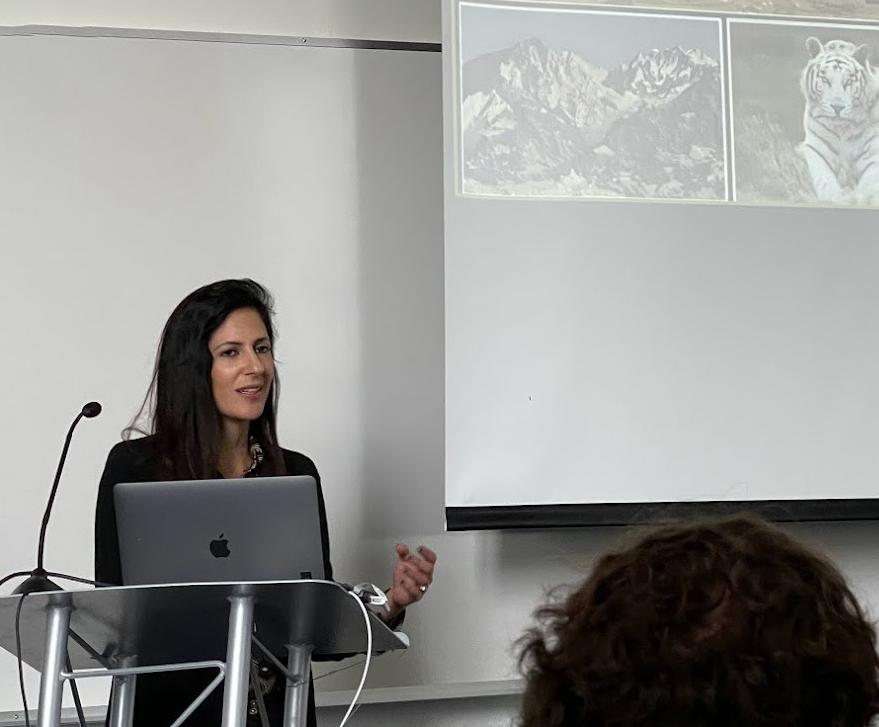
\epsfig{file=figures/how_to_give_talks/speaker.jpg,width=3in}
}
\caption{The key to a good talk:  preparation and practice.}
\label{fig:speaker}
\end{figure}

\noindent We believe the keys to both a good talk and to overcoming nerves are the same: prepare and practice.  Think through your talk.  It's almost always better to give a talk from notes than to read it from a script--the audience feels  you're speaking to them so it's easier for them to pay attention.  But for people giving a talk in a language that they are not comfortable with, writing out a script ahead of time may be a better solution.  There may be parts of the talk that you feel are difficult to get through.  For those parts, even for a native speaker, it may help to write out what you plan to say.  When you give the talk, you may ignore the script, but having written it out once will make it easier to say.

Think through the talk and find the story--how one part relates to the next.  If you can't find that story, you may want to reorder the presentation to create a good story.

When you can, you should visit the room you'll be speaking in to identify any issues that may come up.  Will you be blocking anyone as you stand at the lectern to give the talk?  Will there be someone there to help you set up?  You should decide how to position yourself so that you can see your presentation, and also engage well with the audience.  


\section{Nervousness}

One of us writes, ``I used to be a nervous public speaker.  I still find the hours before giving a presentation to be stressful. I'm always reviewing my talk to try to improve it or to track down the answers to questions I think someone might ask me.  The more I prepare, and the better I know the lecture material, the less stressed I am."

A great cure for nervousness is to practice the talk aloud. Practice by yourself.  Practice in front of your friends.  

One approach \cite{Hoogterp} to calming  nervousness is to remind yourself, 
``Get over it.  They’re not there to see you, they’re there to hear the information.  Just convey the information to them.''

Some find this quote, attributed to Dr. Rob Gilbert \cite{Gilbert}, to be helpful:
``It's all right to have butterflies in your stomach. Your job is to get them to fly in formation.''

\section{Your Distracted Audience}
Before giving a talk, your mental image of the audience may be of many people, listening to your every word.  In reality, on most every speaking situation, your audience is a collection of people who are checking their social media or email, looking on their laptops for other talks to attend, or are hungry or fidgety.  How does one speak to such an audience?  We have to practise and prepare in order to engage the audience.



\section{Ways to Engage the Audience}
In the middle of Patrick Winston's talk about public speaking \cite{WinstonSpeaks}, he asks the audience the question, ``Can you think of a technique to get the audience more engaged in the talk?''  The answer, of course, is to ask them questions.

Bill Hoogterp \cite{Hoogterp} expands on that:  
``The audience is like a sheep dog, always wanting to be working.  Give the audience something to work on while they're listening to you. `Four' pushes people back, while `two plus two' draws them in."  You might pose a sub-problem to them that you had to address in your work, to get them thinking about how to solve that problem.  Then they'll be more receptive to hear your solution.

\subsection{Layer Your Talk}
It's often easier for the audience to listen to your talk if you layer it---provide verbal cues for new concepts and transitions between sections of the talk.  This helps even the attentive listener to follow the structure of your talk.  It keeps the distracted listener from being completely lost.  The distracted listener, only listening for the verbal headings of your talk, may hear,
``The probability of an observation has three terms to it.  $\ldots$ blah blah blah blah $\ldots$
So that gives us the objective function we want to optimize.  Now, how do we find the optimal value?  There are two approaches you can take.  $\ldots$ blah blah blah blah 
So now, with these tools in hand, we can apply this methods to real images. $\ldots$ blah blah blah blah $\ldots$"
Your verbal cues can help even a distracted listener follow your main points.

You can also make your talk easier to follow if you add verbal dynamics---variations in speed or intensity.  Find a part of the talk that is particularly special to you and let that show through.  One of us writes, "When I gave talks about image deblurring, I would emphasize one aspect that I particularly enjoy:
'I love this problem;  it’s beautifully underdetermined.  There are many ways we can explain a blurry image.  It could be that that’s what was there in the world--- we took a sharp picture of a world that happened to look blurry.  Or we took a blurred image of a sharp world.' " The audience loves to watch you be excited about something!


\subsection{People Like to See a Good Fight}

As described by Adelson \cite{Adelson95}, the audience loves to watch a good fight.  You can set up a fight between two competing conjectures.  For example, you might say, ``The flat earth theory predicts that ships will appear on the horizon as small versions of the complete ship.  Under that theory, you’d expect approaching ships to appear as in \fig{\ref{fig:boats}}{a}.  Conversely, the round earth theory predicts that the top of the sails will appear first, then gradually the rest of the ship below it, resulting in approaching ships looking as in \fig{\ref{fig:boats}}{b}.  The audience waits with anticipation as you show them the result from your experiment, \fig{\ref{fig:boats}}{c}, thus revealing the winning theory.

\begin{figure}[htpb!]
\centerline{
\sublabel{a}{
\epsfig{file=figures/how_to_give_talks/boatsflat.jpg,width=1.5in}}
\sublabel{b}{
\epsfig{file=figures/how_to_give_talks/boatsround.jpg,width=1.5in}}
\sublabel{c}{
\epsfig{file=figures/how_to_give_talks/boatsphoto.jpg,width=1.5in}}
}
\caption{(a) The appearance of ships approaching a port, from the flat-earth theory.  (b) Their appearance as predicted by the round-earth theory.  (c) The experimental evidence:  a photograph of ships approaching a port \cite{mnsomero}. }
\label{fig:boats}
\end{figure}



\section{Show Yourself to the Audience}

In a lovely video, the actor Alan Alda describes the importance of  connecting with the audience in scientific presentations \cite{AlanAlda}.  Alda noted the improvement in scientific speaking of volunteers after they engaged in improvisational theater exercises.  After the exercises, the volunteers were primed to engage and connect with others, and their scientific talks sparkled.

Here's what we think an audience wants from a technical talk:
(a) To have one part follow from another and make sense.
(b) To learn a few things.
(c) To connect with the speaker, to share their excitement for the topic. They want to watch you love something!


\subsection{How to End the Talk}
How should you end your talk?  A common, but awkward, way is to end by asking, ``Are there any questions?''  The audience wants to clap at the end of a talk, but with that ending, they don't know whether to applaud or to ask a question, and they're likely to give only scattered applause \cite{Adelson95}.
Better is to close with ``Thank you.''  The audience then knows it's their time to applaud, and they will.  Then you can ask for questions.

We note that Patrick Winston disagrees with ending a talk with "thank you" \cite{WinstonSpeaks}.  He didn't like the implication that the audience was doing you some favor for attending your talk, and preferred to remind the audience of how he has kept his earlier promise to them regarding what they would learn after they listened to his talk.

\section{Concluding Remarks}
Prepare and practice your talks!  As you give the talk, let the audience see how much you enjoy what you've worked on.  Follow-up with the references in this chapter to find the collection of talk tips that works best for you.  Preparation and rehearsal are the best cures we know of for nervousness about giving a talk.


